\documentclass{article}

% Language setting
% Replace `english' with e.g. `spanish' to change the document language
\usepackage[english]{babel}

% Set page size and margins
% Replace `letterpaper' with `a4paper' for UK/EU standard size
\usepackage[letterpaper,top=2cm,bottom=2cm,left=2.5cm,right=2.5cm,marginparwidth=1.8cm]{geometry}

% Useful packages
\usepackage{amsmath}
\usepackage{graphicx}
\usepackage[colorlinks=true, allcolors=blue]{hyperref}
\usepackage{listings}
\usepackage{authblk}

\title{\textbf{Pricing Analysis Platform}}

\usepackage{xcolor}

%New colors defined below
\definecolor{codegreen}{rgb}{0,0.6,0}
\definecolor{codegray}{rgb}{0.5,0.5,0.5}
\definecolor{codepurple}{rgb}{0.58,0,0.82}
\definecolor{backcolour}{rgb}{0.95,0.95,0.92}

%Code listing style named "mystyle"
\lstdefinestyle{mystyle}{
  backgroundcolor=\color{backcolour}, commentstyle=\color{codegreen},
  keywordstyle=\color{purple},
  numberstyle=\tiny\color{codegray},
  stringstyle=\color{codepurple},
  basicstyle=\ttfamily\footnotesize,
  breakatwhitespace=false,         
  breaklines=true,                 
  captionpos=b,                    
  keepspaces=true,                 
  numbers=left,                    
  numbersep=5pt,                  
  showspaces=false,                
  showstringspaces=false,
  showtabs=false,                  
  tabsize=2
}

%"mystyle" code listing set
\lstset{style=mystyle}

\author{Bruno Campos U., Iván Serrano Z., Luis Noguera G., Maximino Navarro M. 
\\ José María Sarmiento Chávez}
\affil[]{Universidad Panamericana 
\\Maestría en Ciencia de Datos}

\begin{document}

\begin{figure}

\includegraphics[width=0.4\linewidth]{Reports/images/up_logo.jpg}
\end{figure}

\maketitle

\section{Resumen Ejecutivo}

En este trabajo se plantea la propuesta de crear una plataforma para \textbf{analizar} y \textbf{predecir} los precios de la canasta básica alimentaria, utilizando datos de "Quién es Quién en los Precios" de la Profeco y herramientas como \textbf{Hadoop}, \textbf{Spark}, \textbf{python} y \textbf{Google Cloud Platform}. El objetivo es mejorar la capacidad de planificación de compras informadas para los consumidores, mediante la generación de modelos predictivos que permitan anticipar las fluctuaciones de precios. Esto no solo proporcionará a los consumidores una herramienta estratégica para la gestión de su presupuesto, sino que también contribuirá a resolver problemas socioeconómicos al brindar información valiosa para la formulación de políticas públicas orientadas a garantizar el acceso a alimentos asequibles y promover el bienestar económico de la población. El uso del \textbf{Big Data} en este contexto no solo permite comprender las tendencias históricas de precios, sino también identificar patrones predictivos que pueden ser utilizados para anticipar las fluctuaciones futuras, ofreciendo así una visión más clara y anticipada de la dinámica de precios en el mercado de alimentos básicos.

\subsection{Introducción}

En México, se han llevado a cabo importantes trabajos con el objetivo de definir una canasta que refleje las necesidades básicas de los mexicanos. Entre ellos, destacan la Canasta Normativa de Satisfactores Esenciales (CNSE), la Canasta Alimentaria propuesta por la Comisión Económica para América Latina y el Caribe (CEPAL) en colaboración con el INEGI, y las canastas Alimentaria y No Alimentaria del CONEVAL.\\

La CNSE se desarrolló a partir de la Encuesta de Ingresos y Gastos Familiares de 1975 del Centro Nacional de Información y Estadísticas del Trabajo, con el objetivo de reflejar los patrones de consumo frecuentes en la población mexicana, así como cumplir con las normativas y objetivos establecidos por la legislación mexicana.\\

La Canasta Alimentaria, creada por el CEPAL y el INEGI en 1998, tuvo como propósito reflejar las necesidades nutricionales de la población mexicana. Esta iniciativa formó parte de un esfuerzo más amplio para homogeneizar la metodología de medición de la pobreza en América Latina.\\

Posteriormente, en 2004, la Ley General de Desarrollo Social (LGDS) estableció la creación del CONEVAL con el fin de normar y coordinar la evaluación de políticas y programas de desarrollo social, así como definir, identificar y medir la pobreza. En 2010, el CONEVAL publicó una canasta alimentaria para los ámbitos rural y urbano, adaptando la metodología desarrollada por la CEPAL y el INEGI, así como una canasta no alimentaria basada en la propuesta metodológica de Hernández Laos. Estas canastas fueron diseñadas para medir la pobreza multidimensional, una de las funciones principales del CONEVAL.\\

La Procuraduría Federal del Consumidor (Profeco) recopila los precios de 200 000 productos específicos en aproximadamente 1 500 establecimientos comerciales, productos que representan alrededor de 3 600 marcas, variedades y presentaciones. Estos precios son presentados a través de un programa denominado “Canasta Inteligente”, que permite al usuario crear su propia canasta en función de sus necesidades, a fin de darle a conocer los precios mínimos y promedio, así como el mejor lugar de compra. Asimismo, se presentan catálogos que asocian un conjunto de productos con base en la Canasta Básica y la información de gasto de la Encuesta Nacional de Ingresos y Gastos de los Hogares que realiza el INEGI. 


\section{Visión general del desarrollo}

En este trabajo se plantea la propuesta de crear una plataforma para \textbf{analizar} y \textbf{predecir} los precios de la canasta básica alimentaria, utilizando datos de "Quién es Quién en los Precios" de la Profeco y herramientas como \textbf{Hadoop}, \textbf{Spark}, \textbf{python} y \textbf{Google Cloud Platform} para gestionar el gran volumen de información que se necesita para crear un sistema robusto y crear los modelos que permitan realizar la predicción de precios. \\

El objetivo que se busca con este proyecto, es el mejorar la capacidad de planificación de compras para los consumidores, mediante la generación de pronósticos que permitan anticipar las fluctuaciones de precios. Este enfoque no solo proporcionará a los consumidores una herramienta estratégica para la gestión de su presupuesto, sino que también contribuirá a resolver problemas socioeconómicos al brindar información valiosa para la formulación de políticas públicas orientadas a garantizar el acceso a alimentos asequibles y promover el bienestar económico de la población. \\

El uso del \textbf{Big Data} en este contexto no solo permite comprender las tendencias históricas de precios, sino también identificar patrones predictivos que pueden ser utilizados para anticipar las fluctuaciones futuras, ofreciendo así una visión más clara y anticipada de la dinámica de precios en el mercado de alimentos básicos.

\subsection{Solución Actual}
Actualmente la Profeco realiza un seguimiento quicenal de los precios de un listado de productos básicos y de alto consumo para la alimentación de la población mexicana a través de su programa llamado  \href{https://www.profeco.gob.mx/precios/canasta/qqpc.php}{Quién es Quién en los precios (QQP)}. En el portal de QQP podrémos encontrar la siguiente descripción acerca de qué es lo que hace:\\

\begin{enumerate}
\item El programa Quién es Quién en los Precios (QQP) recopila y difunde información sobre precios de productos domésticos de consumo habitual, como alimentos, bebidas, productos de cuidado personal, artículos para el hogar, medicamentos, electrodomésticos y artículos de temporada. Esta información tiene como objetivo ayudarle a tomar decisiones de compra informadas mediante la comparación de precios.

\item Los precios se recogen visitando una muestra de los principales establecimientos de cada una de las ciudades participantes en el programa durante los cinco días hábiles de la semana.

\item  Los precios mostrados incluyen la fecha en que fueron tomados; sin embargo, están sujetos a cambios ya que algunos establecimientos pueden variar sus precios más de una vez al día. Por tanto, deben considerarse precios de referencia.

\end{enumerate}

Poder contar con estos datos es indipensable para analizar la variación en los precios de estos productos y saber cómo dichas variaciones de precios podrían impactar a los consumidores finales.\\

La Profeco, además de dar un seguimiento quicenal a los precios de los productos, genera un reporte semanal de los precios máximos y mínimos de una canasta de 24 alimentos (ver figura 1) que fueron tomandos de la canasta alimentaria definida por el CONEVAL y muestra dicho análisis por las distintas regiones de México (las regiones definidas por El Banco de México (BANXICO) en su Reporte sobre las economías regionales, julio-septiembre 2021).

\begin{figure}[h]
\centering
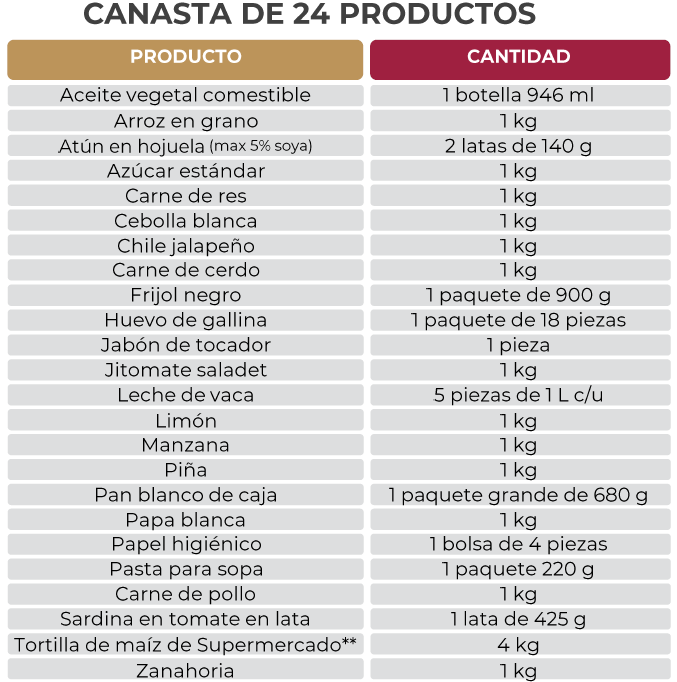
\includegraphics[width=0.5\linewidth]{Reports/images/Canasta.png}
\caption{\label{fig:Architecture}Canasta Básica de 24 productos}
\end{figure}

En el reporte que genera el programa QQP se muestran las tendencias de los precios del grupo de alimentos en estudio (los 24 alimentos que conforman la canasta) (ver figura 2), pero se muestran dos líneas: una línea corresponde al precio mínimo en el que se puede comprar dicha canasta y la otra línea muestra el precio máximo.Por otro lado, estos valores se comparan con el Índice Nacional de Precios al Consumidor (INPC) que actualmente está conformado por una canasta de 299 productos y servicios, para tenerlo como referencia.\\

Un Índice de Precios al Consumidor es un indicador económico que mide, a lo largo del tiempo, la variación promedio de los precios de una canasta de bienes y servicios representativa del consumo de los hogares del país.

\begin{figure}[h]
\centering
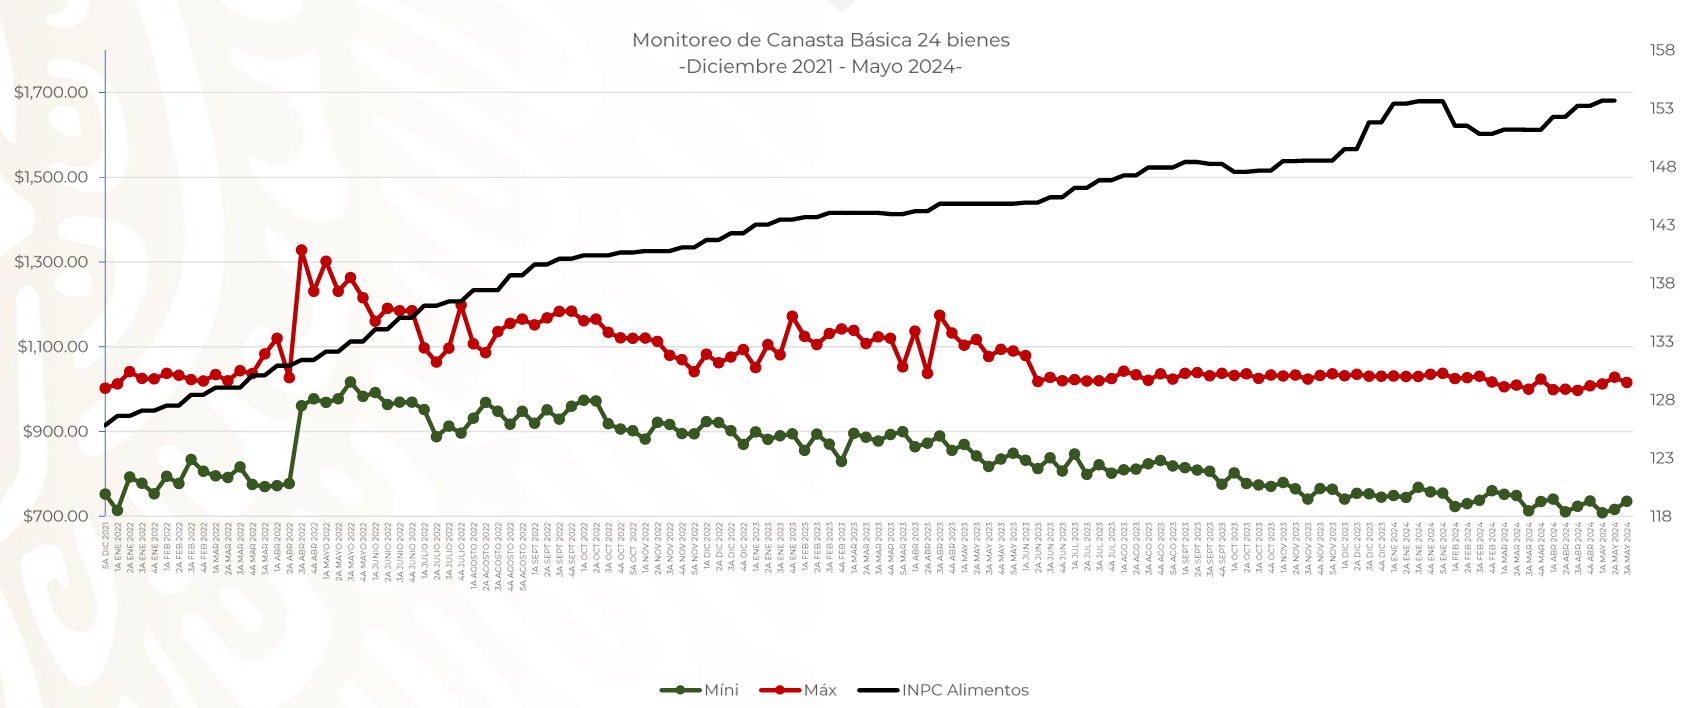
\includegraphics[width=0.7\linewidth]{Reports/images/Tendencia.png}
\caption{\label{fig:Canasta}Tendencia de precios máximos y mínimos de las canasta básica vs el INPC}
\end{figure} 

\newpage
\subsection{Limitaciones actuales de la solución}

La primera idea que se tuvo acerca de este proyecto era la de crear una plataforma que funcionara en tiempo real. Sin embargo, actualmente no se cuenta con sistemas que brinden información con las características que se requieren para que sea un proyecto que deba ser solucionado con dicho enfoque. Recordemos que para los proyectos de Big data re requiere que se cumplan las tres v: volumen, variedad y velocidad. La última v, que corresponde a la velocidad, es la que nos impide crear un sistema que funcione en tiempo real, puesto que los datos se actualizan cada 15 días (a pesar de extraerse de forma diaria, de lunes a viernes). 

\subsection{Propósito, uso y alcance de la herramienta}
    
El propósito de reporte de \textbf{QQP} es mostrar la información con el detalle del establecimiento, la entidad, municipio, domicilio y el precio de referencia (ver figura 3) para que los consumidores puedan estar realizar comparaciones y realizar sus compras de manera más informada (justo como se informa en la página del programa). Entonces el alcance sería prácticamente ese, el de servir como una referencia del precio de la canasta básica en las regiones correspondientes. 

\begin{figure}[h]
\centering
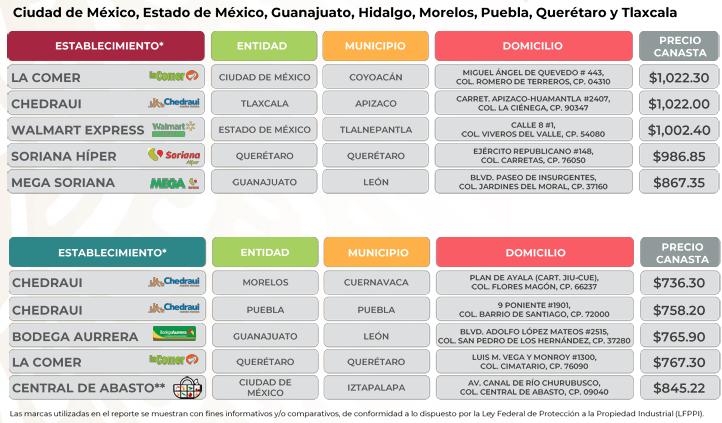
\includegraphics[width=0.9\linewidth]{images/Top 5.png}
\caption{\label{fig:Canasta}Top 5 de los precios mínimos y máximos en la región centro del país}
\end{figure}

El enfoque y propósito de nuestra solución sería mostrar la información de manera desagregada y por ciudad, ya que se esta manera se complementaría con lo que ya se informa en el programa, pero a un nivel de detalle mayor. Adicionalmente, el alcance actual del reporte de QQP solo es de caracter informativo, sin embargo, es necesario ir más allá para que realmente la herramienta pueda 

\newpage
\section{Revisión y uso de datos}

\subsection{Orígenes y control de datos}

Los datos son extraídos como archivo por archivo a través de un proceso de web scrapping usando python, de la página de datos abiertos de Profeco \verb|https://datos.profeco.gob.mx/datos_abiertos/qqp.php| (ver figura 4). Este proceso se describe con mayor detalle en la sección de \textbf{Extracción, Carga y Transformación de datos}. 


\begin{figure}[h]
\centering
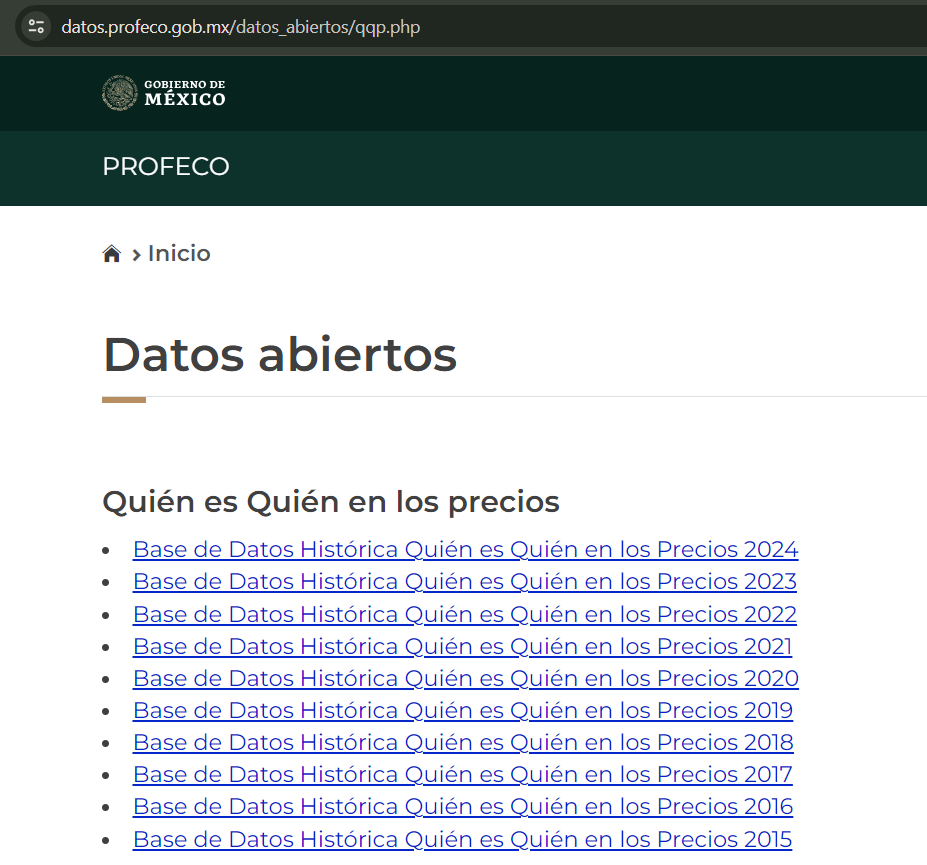
\includegraphics[width=1\linewidth]{Reports/images/datos.png}
\caption{\label{fig:datos} Ligas para la extracción de los datos}
\end{figure}

\newpage
Los datos de QQP consisten en un listado que contiene el detalle de Producto, Presentación, Marca, Categoría, Precio, Cadena comercial, hasta Latitud y Longitud del negocio (ver figura 5).

\begin{figure}[h]
\centering
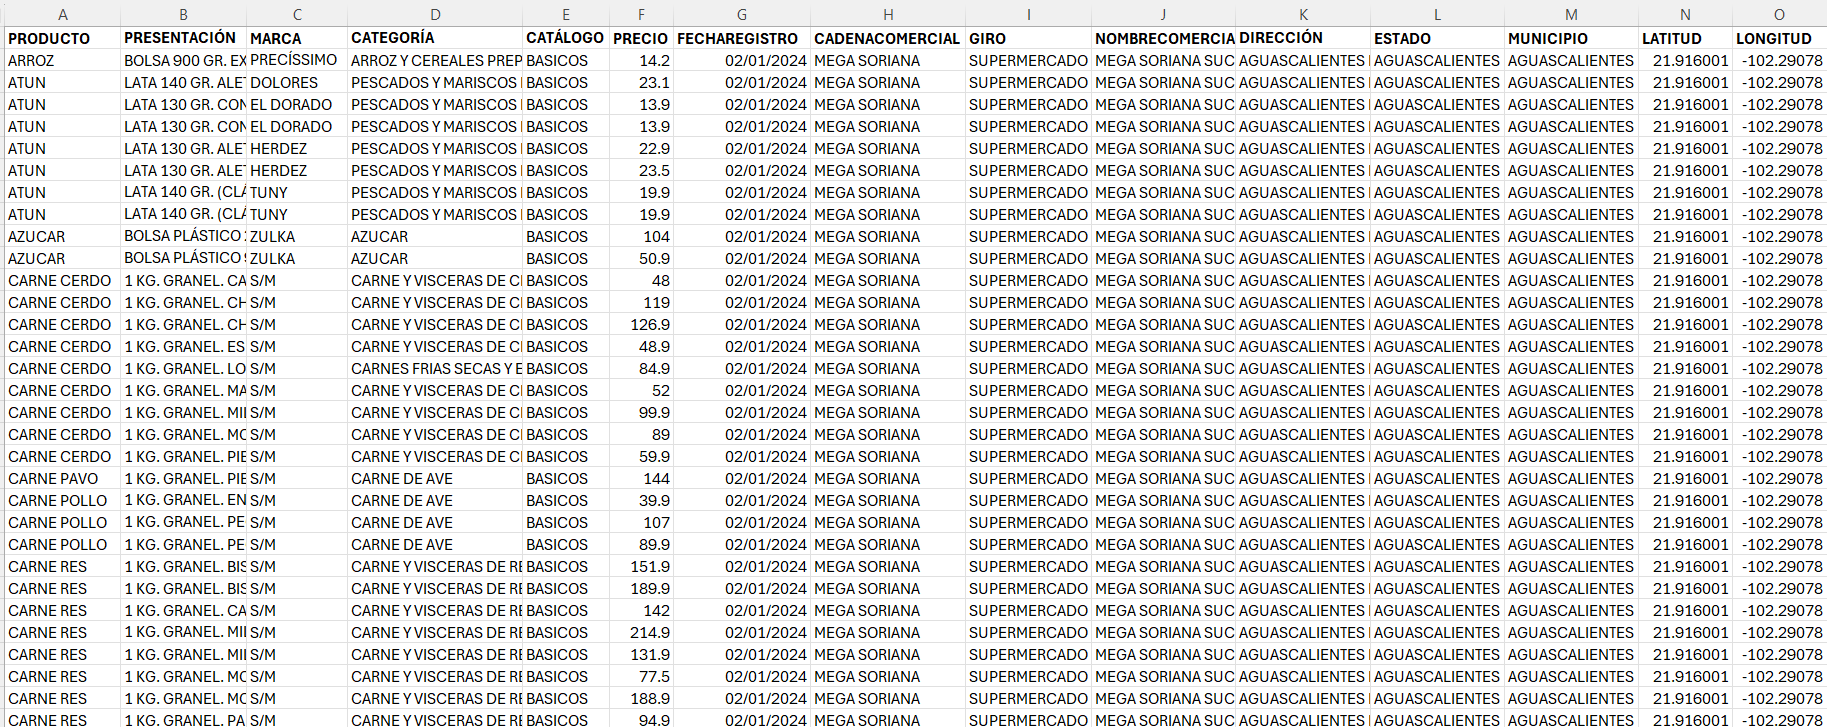
\includegraphics[width=1\linewidth]{Reports/images/sample.png}
\caption{\label{fig:sample} Vista de los campos contenidos en los archivos csv de QQP}
\end{figure}
\subsection{Preparación de los datos}

La preparación de los datos se describe con mayor detalle en la sección de ELT, en donde se muestran el proceso de Extracción, Carga y Transformación de los datos. 

\subsection{Limpieza y tratamiento de datos}

La limpieza de los datos consistió en la eliminación de los Outliers de los registros ya filtrados para la generación del modelo de predicción. Dicho proceso viene incluido y mejor explicado en la sección del forecast. 

\subsection{Integridad de los datos}


HDFS asegura la integridad de los datos mediante la replicación de bloques. Cada archivo en HDFS se divide en bloques, y cada bloque se replica en varios nodos (por defecto, tres). Esto significa que si uno de los nodos falla, las réplicas en otros nodos garantizan la disponibilidad y la integridad de los datos. HIVE está diseñado para integrarse estrechamente con HDFS, aprovechando todas las características de integridad y fiabilidad de HDFS. Esto significa que cualquier archivo almacenado y gestionado por HIVE en HDFS se beneficia automáticamente de las garantías de integridad de HDFS.

Al usar spark mediante python (pyspark) y al tener datasets una misma estructura, es posible cargar la información de una manera limpia, ya que es posible definir la estructura de la tabla con la estructura de los datos. 


\subsection{Limitaciones de los datos}

Como ya se mencionó anteriormente, los datos son recolectados semana tras semanas, pero publicados cada 15 días a través de la plataforma de QQP, esa es una de las principales limitaciones de la información, ya que se podría obtener una plataforma más robusta si los datos se extrayeran diariamente, de tal manera que se pudiera observar la variación diaria.
Otra limitación tiene ver con el hecho de que no se extraen los datos de todos los días de la semana. Esto sugiere un problema, pues si suponenmos que la gente hace sus compras principalmente los fines de semana, no estaríamos logrando capturar las variaciones en los precios en dichos días. La razón principal de suponer esto como un problema, tiene que ver con que la demanda de los productos afecta directamente a su precio, por lo tanto estaríamos perdiendo ese importante efecto en los precios. 

\section{Proceso de desarrollo}

\subsection{Metodología}
La metodología CRISP-DM (Cross Industry Standard Process for Data Mining) es un modelo estándar ampliamente utilizado en la minería de datos y en el campo de la ciencia de datos. Proporciona un marco estructurado para planificar y ejecutar proyectos de minería de datos, y se compone de seis fases principales:

\begin{enumerate}
\item \textbf{Comprensión del Negocio (Business Understanding):}

\begin{itemize}
\item Objetivo: Entender los objetivos y requisitos del proyecto desde una perspectiva de negocio.
\item Tareas: Definir los objetivos del negocio, evaluar la situación actual, definir los objetivos de minería de datos y producir un plan de proyecto.
\end{itemize}

\item \textbf{Comprensión de los Datos (Data Understanding):}

\begin{itemize}
\item Objetivo: Familiarizarse con los datos y evaluar su calidad.
\item Tareas: Recolectar datos iniciales, describir los datos, explorar los datos y verificar la calidad de los datos.
\end{itemize}

\item \textbf{Preparación de los Datos (Data Preparation):}

\begin{itemize}
\item Objetivo: Preparar los datos en una forma que pueda ser utilizada para el modelado.
\item Tareas: Selección de datos, limpieza de datos, construcción de datos, integración de datos y formateo de datos.
\end{itemize}

\item \textbf{Modelado (Modeling):}

\begin{itemize}
\item Objetivo: Aplicar técnicas de modelado para crear modelos que puedan cumplir con los objetivos del proyecto.
\item Tareas: Selección de técnicas de modelado, generación de diseño de pruebas, creación de modelos y evaluación de los modelos.
\end{itemize}

\item \textbf{Evaluación (Evaluation):}

\begin{itemize}
\item Objetivo: Evaluar los modelos para asegurarse de que cumplen con los objetivos del negocio.
\item Tareas: Evaluar los resultados, revisar el proceso y determinar los próximos pasos.
\end{itemize}

\item \textbf{Despliegue (Deployment):}

\begin{itemize}
\item Objetivo: Implementar los modelos en un entorno de producción para que puedan ser utilizados en la toma de decisiones.
\item Tareas: Planificación de la implementación, monitoreo y mantenimiento del modelo, creación de informes finales y revisión del proyecto.
\end{itemize}
\end{enumerate}

\begin{figure}[h]
\centering
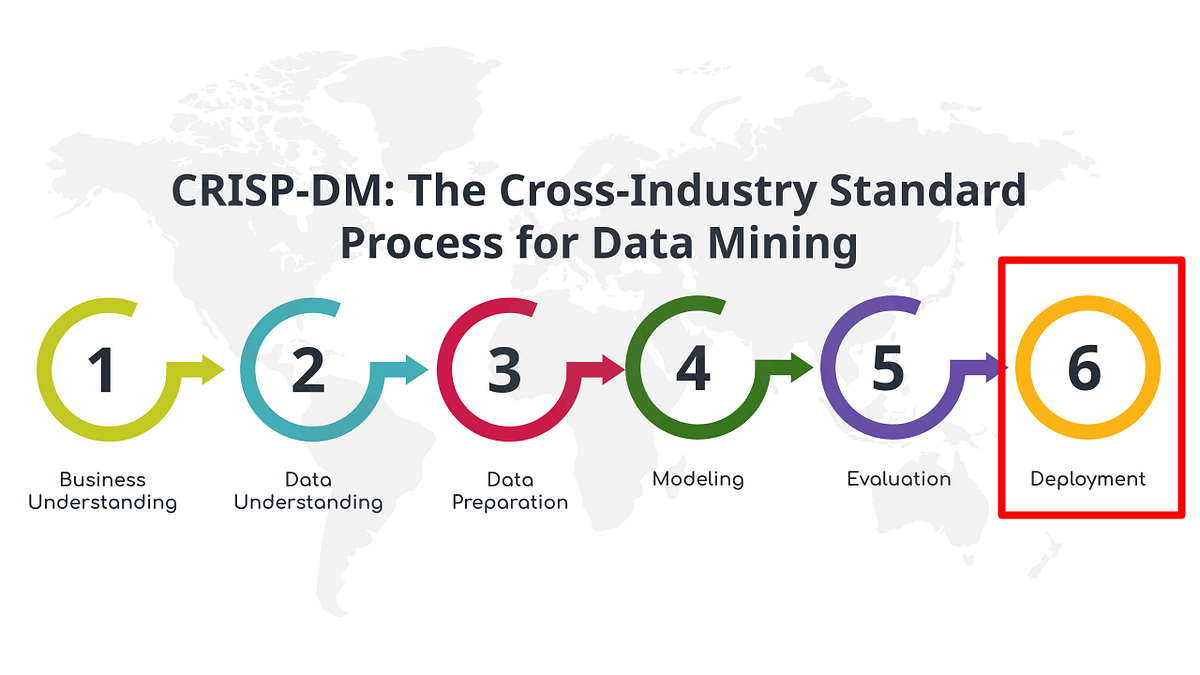
\includegraphics[width=0.75\linewidth]{images/CRISP-DM.png}
\caption{\label{fig:Canasta}La metodología CRISP-DM (Cross Industry Standard Process for Data Mining)}
\end{figure}

\subsection{Preparación de los entornos de trabajo}

En esta sección se integran los códigos y procesos que se llevaron a cabo para levantar la instancia de María DB que posteriormente se ocuparía para la carga de los datos agregados.

\subsubsection{Creación de la instancia en GCP}

Guía de instalación (esta guía también la podrás encontrar dentro del archivo README.md en la siguiente ruta dentro del github del proyecto: \href{https://github.com/Anonymate054/MCD-BigData/tree/main/GCP/compute-engine/mariadb_shells}{GCP/compute-engine/mariadb_shells} .

\textbf{Create an instance on GCP 'Compute Engine'}

\textit{Equivalent code (in process):}


\begin{lstlisting}[language=bash,caption={bash version}]
```
gcloud compute instances create <instance_name> --project=<project_name> --zone=us-central1-a --machine-type=e2-medium --network-interface=network-tier=PREMIUM,stack-type=IPV4_ONLY,subnet=default --maintenance-policy=MIGRATE --provisioning-model=STANDARD --service-account=620836759706-compute@developer.gserviceaccount.com --scopes=https://www.googleapis.com/auth/cloud-platform --tags=http-server,https-server,lb-health-check --create-disk=auto-delete=yes,boot=yes,device-name=<instance_name>,image=projects/ubuntu-os-cloud/global/images/ubuntu-2004-focal-v20240515,mode=rw,size=80,type=projects/bigdata2-423718/zones/us-central1-a/diskTypes/pd-balanced --no-shielded-secure-boot --shielded-vtpm --shielded-integrity-monitoring --labels=goog-ec-src=vm_add-gcloud --reservation-affinity=any
```
\end{lstlisting}

\begin{lstlisting}[language=bash,caption={bash version}]
```
gcloud compute instances create <instance_name> \
    --project=<project-name> \
    --zone=us-central1-a \
    --machine-type=e2-medium \
    --network-interface=network-tier=PREMIUM,stack-type=IPV4_ONLY,subnet=default \
    --maintenance-policy=MIGRATE \
    --provisioning-model=STANDARD \
    --service-account=<service_account>-compute@developer.gserviceaccount.com \
    --scopes=https://www.googleapis.com/auth/cloud-platform \
    --tags=http-server,https-server,lb-health-check \
    --create-disk=auto-delete=yes,boot=yes,device-name=instance-20240529-231717,image=projects/ubuntu-os-cloud/global/images/ubuntu-2004-focal-v20240519,mode=rw,size=10,type=projects/<project_name>/zones/us-central1-a/diskTypes/pd-balanced \
    --no-shielded-secure-boot \
    --shielded-vtpm \
    --shielded-integrity-monitoring \
    --labels=goog-ec-src=vm_add-gcloud \
    --reservation-affinity=any
```
\end{lstlisting}

\textbf{Cloning a Single Directory from a GitHub Repository}
You can clone a single directory from a GitHub repository by using a combination of Git sparse-checkout and filter features. Follow these steps:

\begin{lstlisting}[language=bash,caption={bash version}]

1. **Update and upgrade system**
    ```bash
    sudo apt get update
    sudo apt get upgrade
    ```

2. **Create filename**
    ```bash
    mkdir codes
    cd codes
    ```

3. **Initialize a new Git repository:**
    ```bash
    git init
    ```

4. **Add the remote repository::**
    ```bash
    git remote add origin https://github.com/Anonymate054/MCD-BigData.git
    ```

5. **Enable the sparse-checkout feature:**
    ```bash
    git config core.sparseCheckout true
    ```

6. **Specify the directory you want to clone:**
    ```bash
    echo "GCP/compute-engine/mariadb_shells/*" >> .git/info/sparse-checkout
    ```

7. **Pull the specified directory from the remote repository:**
    ```bash
    git pull origin main
    ```
\end{lstlisting}

\subsubsection{Creación de la instancia de MaríaDB}

\textbf{Instalations of mariadb}
\begin{lstlisting}[language=bash,caption={bash version}]
1. **Move to files:**
    ```bash
    cd GCP/compute-engine/mariadb_shells
    ```

2. **Grand persitions:**
    ```bash
    chmod +x 1_instalar_mariadb_easy.sh
    ```

3. **Run script:**
    ```bash
    sudo ./1_instalar_mariadb_easy.sh
    ```

4. **Create user root:**
    Follow instructions, for root password, press enter (since it's the first time) and then set a new one, in this case Example123, everything else `YES` or `y`.

5. **Check if the system is running:**
    ```bash
    sudo systemctl status mariadb
    ```

6. **Grand persitions:**
    ```bash
    chmod +x 2_crear_usuario.sh
    ```

7. **Run script:**
    ```bash
    sudo ./2_crear_usuario.sh
    ```

8. **Test connection**
    ```bash
    mysql -u big_data_user -p
    ```
    
9. **Grand persitions:**
    ```bash
    chmod +x 3_modificar_configuracion.sh
    ```

10. **Run script:**
    ```bash
    sudo ./3_modificar_configuracion.sh
    ```

11. **Grand persitions:**
    ```bash
    chmod +x 4_crear_regla_vpc.sh
    ```

12. **Run script:**
    ```bash
    sudo ./4_crear_regla_vpc.sh
    ```

13. **Reboot system:**
    ```bash
    sudo reboot
    ```
\end{lstlisting}


\textbf{Creación de la base de datos QQP en MariaDB y creación de la tabla} \verb|QQP_AGGREGATED|
\begin{lstlisting}[language=sql,caption={sql version}]
1. **Create Database**
```sql
MariaDB [(none)]> CREATE DATABASE QQP;
```

2. **Create Table:**

```sql
MariaDB [(none)]> USE QQP;
MariaDB [QQP]> CREATE TABLE QQP.aggregated (
  `fecha` longtext DEFAULT NULL,
  `fecha_year` int(11) DEFAULT NULL,
  `fecha_month` int(11) DEFAULT NULL,
  `producto` longtext DEFAULT NULL,
  `descripcion` longtext DEFAULT NULL,
  `count_marca` bigint(20) NOT NULL,
  `count_tiendas` bigint(20) NOT NULL,
  `count_estados` bigint(20) NOT NULL,
  `count_municipios` bigint(20) NOT NULL,
  `precio_avg` decimal(22,6) DEFAULT NULL,
  `precio_desv_std` double DEFAULT NULL,
  `precio_median` decimal(18,2) DEFAULT NULL,
  `precio_max` decimal(18,2) DEFAULT NULL,
  `precio_min` decimal(18,2) DEFAULT NULL
);
```
\end{lstlisting}

\subsubsection{Creación de clúster en Dataproc}

Guía de instalación (esta guía también la podrás encontrar dentro del archivo README.md en la siguiente ruta dentro del github del proyecto: \href{https://github.com/Anonymate054/MCD-BigData/tree/main/GCP/dataproc}{GCP/dataproc}.\\

\textbf{Google Cloud SDK Installation}
Para utilizar Google Cloud SDK para su proyecto, siga estos pasos para instalarlo y configurarlo en un sistema Linux. Para otros sistemas operativos, consulte la [guía de instalación oficial](https://cloud.google.com/sdk/docs/install).\\

\textit{\textbf{Nota}: en dado caso de que falle al ejecución desde shell, realizar la operación de manera manual. Se está trabajando en la optimización y automatización de los scripts.} \\

\textbf{Step-by-Step Installation}

\begin{lstlisting}[language=sql,caption={bash version}]
1. **Download Google Cloud SDK:**

   Run the following command to download the Linux archive file:

   ```bash
   curl -O https://dl.google.com/dl/cloudsdk/channels/rapid/downloads/google-cloud-cli-477.0.0-linux-x86_64.tar.gz
    ```

2. **Uncompress the Files:** 

    Unpack the downloaded archive using the following command:

   ``` bash
   ./google-cloud-sdk/install.sh
    ```

3. **Install Google Cloud SDK:**

    Navigate to the extracted directory and run the installation script:

   ``` bash
   ./google-cloud-sdk/install.sh
    ```

    During installation, you will see the following text:

    ``` bash
    Welcome to the Google Cloud CLI!

    To help improve the quality of this product, we collect anonymized usage data
    and anonymized stacktraces when crashes are encountered; additional information
    is available at <https://cloud.google.com/sdk/usage-statistics>. This data is
    handled in accordance with our privacy policy
    <https://cloud.google.com/terms/cloud-privacy-notice>. You may choose to opt in this
    collection now (by choosing 'Y' at the below prompt), or at any time in the
    future by running the following command:

        gcloud config set disable_usage_reporting false

    Do you want to help improve the Google Cloud CLI (y/N)?  y


    Your current Google Cloud CLI version is: 477.0.0
    The latest available version is: 477.0.0
    ```
    Follow the prompts to complete the installation. You may choose to opt-in or out of data collection.

4. Initialize Google Cloud SDK:

    After installation, initialize the SDK:

   ``` bash
   ./google-cloud-sdk/bin/gcloud init
    ```

    This command will guide you through the initial setup, including logging in with your Google account and selecting a Google Cloud project.

    ``` bash 
    Welcome! This command will take you through the configuration of gcloud.

    Your current configuration has been set to: [default]

    You can skip diagnostics next time by using the following flag:
    gcloud init --skip-diagnostics

    Network diagnostic detects and fixes local network connection issues.
    Checking network connection...done.
    Reachability Check passed.
    Network diagnostic passed (1/1 checks passed).

    You must log in to continue. Would you like to log in (Y/n)?  y
    ```

    Follow the prompts to log in, select a cloud project, and configure a default compute region and zone if desired.

    ``` bash
    Pick cloud project to use:
    [1] bigdata-#####
    [2] Create a new project
    Please enter numeric choice or text value (must exactly match list item):  2

    Your current project has been set to: [bigdata-#####].

    Do you want to configure a default Compute Region and Zone? (Y/n)?  y

    ```
For more detailed information please visit the [Install the gcloud CLI ](https://cloud.google.com/sdk/docs/install)
## Post-Installation Configuration

After installation and initial configuration, you might want to install additional components or update your SDK:

1. **Install/Remove Components:**

    ``` bash
    gcloud components install COMPONENT_ID
    gcloud components remove COMPONENT_ID
    ```

2. **Update SDK to the Latest Version:**

    ``` bash
    gcloud components update
    ```

Modify Profile to Update PATH and Enable Shell Command Completion:
Follow the prompts to modify your shell profile (e.g., `.bashrc`, `.zshrc`).

For more detailed information and advanced configuration options, please visit the [Google Cloud SDK Quickstarts](https://cloud.google.com/storage/docs/gsutil/commands/config).


# Create a new project

1. **Create a New Project**: Execute the following command to create a new project:

   ```bash
   gcloud projects create <project-id>
   ```
   *Example:* `gcloud projects create bigdata-qqp2`

2. **List Projects:** To list all projects, use:
   ```bash
   gcloud projects list
   ```

3. **Check Current Project:** To see which project you're currently working on, use:
   ```bash
   gcloud config list project
   ```

4. **Change Project:** To switch to a different project, use:
   ```bash
   gcloud config set project <project-id>
   ```
   *Example:*`gcloud config set project bigdata-qqp2`

## Resolving Billing Account Issue

To resolve the billing account issue, follow these steps:

1. **Verify Billing Account**: Ensure that your project has a billing account associated with it. You can do this by using the following command:

   ```bash
   gcloud beta billing accounts list
   ```
   This will display a list of available billing accounts and their IDs. If you don't have a billing account associated, you'll need to create one in the Google Cloud Billing console.

2. **Associate Billing Account with Project:**: If you have a billing account available, you can associate it with your project using the following command:

    ```bash
    gcloud beta billing projects link <project-id> --billing-account=<billing-account-id>
    ```
    Replace `<project-id>` with your project's ID and `<billing-account-id>` with the ID of the billing account you wish to associate.

Once you have associated a billing account with the project, try enabling the Dataproc service again using the following command:

```bash
gcloud services enable dataproc.googleapis.com --project=<project-id>
```

If the billing account is properly configured, the Dataproc service should be able to activate without any issues.

# Create a new instance of Dataproc

## Manual instalation

You can create a new instance of Dataproc using the following command:

    gcloud dataproc clusters create <cluster-name> --enable-component-gateway --region <region> --subnet default --master-machine-type e2-standard-4 --master-boot-disk-size 100 --num-workers 2 --worker-machine-type n2-standard-2 --worker-boot-disk-size 200 --image-version 2.2-ubuntu22 --optional-components JUPYTER,ZEPPELIN,DOCKER --scopes 'https://www.googleapis.com/auth/cloud-platform' --project <project-name>
    

Make sure to replace `<cluster-name>`, `<region>`, `<project-name>` with your actual information.

## Semi-automatic installation

Alternatively, you can execute the `create_cluster.sh` script by providing three parameters: `cluster name`, `region`, and `project name`.

1. **Grant permission to the script:**

    ``` bash
    chmod +x ./create_cluster.sh
    ```

2. **Create cluster:**

    ``` bash
    ./create_cluster.sh -n my-cluster -r us-east1 -p my-project
    ```
    *Example:* `./create_cluster.sh -n cluster-qqp -r us-east1 -p bigdata-qqp2`

## Gran permissions to GCP IAM

If you encounter an error while creating the cluster regarding permissions, follow these steps.

1. **Grant permission to the script:**

    ``` bash
\end{lstlisting}

\subsubsection{Extracción, Carga y Transformación de datos (ELT)}

Para la extracción de los datos se hizo mediante un scrapper desarrollado en python usando las siguientes bibliotecas:\\
\begin{lstlisting}[language=Python]
    from lxml import html
    import requests
    import re
    import os
\end{lstlisting}

Se entra a la página de QQP \textit{https://www.profeco.gob.mx/precios/canasta/qqpc.php} y se hace todo el procedimiento de exploración y extracción de distintas partes de la página para encontrar las secciones de HTML que contienen los archivos csv. Después se crea un proceso que extraerá uno por uno los archivos que fueron cargados de forma quicenal y se guardan en carpetas con el nombre del mes, año y la quincena a la que corresponde en archivos rar. 

\begin{lstlisting}[language=Python, caption={python version}]

page=requests.get('https://datos.profeco.gob.mx/datos_abiertos/qqp.php')
tree = html.fromstring(page.content)

links = tree.xpath('/html/body/main/div/div//@href')

names = tree.xpath('/html/body/main/div/div//a/text()')

clean_year = ['QQP_'+re.findall(r'\d+',s)[0] for s in names]

pages = dict(zip(clean_year,links))

def create_folder_if_not_exists(folder_name):
    if not os.path.exists(folder_name):
        os.makedirs(folder_name)
        print(f"The folder '{folder_name}' has been created.")
    else:
        print(f"The folder '{folder_name}' already exists.")

for year in pages:
    print(year, "->", pages[year])

home = 'https://datos.profeco.gob.mx/datos_abiertos/'

def download_files(home, json_pages):
    for year in json_pages:
        url = home + json_pages[year]
        print('Trying to download {} -> {}'.format(url, year))
        try:
            response = requests.get(url)
            if response.status_code == 200:
                create_folder_if_not_exists("files/{year}".format(year = year))
                with open("files/{year}/{year}.rar".format(year = year), "wb") as file:
                    file.write(response.content)
                    print("File downloaded successfully!")
            else:
                print("Failed to download the file.")
        except Exception as e:
                print(f"Failed to open the menu. \n Error: {e}")
download_files(home, pages)
\end{lstlisting}

Posteriormente se ejecuta el script para la descompresión de los archivos rar.

\begin{lstlisting}[language=bash,caption={bash version}]
#!/bin/bash

# Instalar rar y unrar si no estan instalados
sudo apt update && sudo apt upgrade -y
sudo apt install -y rar unrar

# Obtener el directorio base desde el argumento de la linea de comandos
base_dir="$1"

# Verificar si se proporciona un directorio base
if [ -z "$base_dir" ]; then
  echo "Uso: $0 <directorio>"
  exit 1
fi

# Verificar si el directorio base existe
if [ ! -d "$base_dir" ]; then
  echo "El directorio base '$base_dir' no existe."
  exit 1
fi

# Listar todos los directorios en el directorio base
for dir in "$base_dir"/*; do
  if [ -d "$dir" ]; then
    # Extraer el nombre del directorio
    dir_name=$(basename "$dir")
    
    # Definir la ruta del archivo .rar
    rar_file="$dir/$dir_name.rar"
    
    # Definir el directorio de salida csv
    csv_dir="$dir/csv"
    
    # Crear el directorio csv si no existe
    mkdir -p "$csv_dir"
    
    # Extraer el archivo .rar en el directorio csv
    unrar e "$rar_file" "$csv_dir"
  fi
done
\end{lstlisting}

Para más detalle de cómo realizar la extracción de los datos, remitirse a la sección correspondiente de \textit{Data Extraction and Analysis Platform} \href{https://github.com/Anonymate054/MCD-BigData/tree/main/Scrapper}{MCD-BigData/tree/main/Scrapper} (ver figura 7), dentro del Github del proyecto y seleccionar el archivo \textit{Scrapper.ipynb} que se encuentra dentro de la siguiente ruta: \textit{Scrapper/notebooks/Python-classic/}.


\begin{figure}[h]
\centering
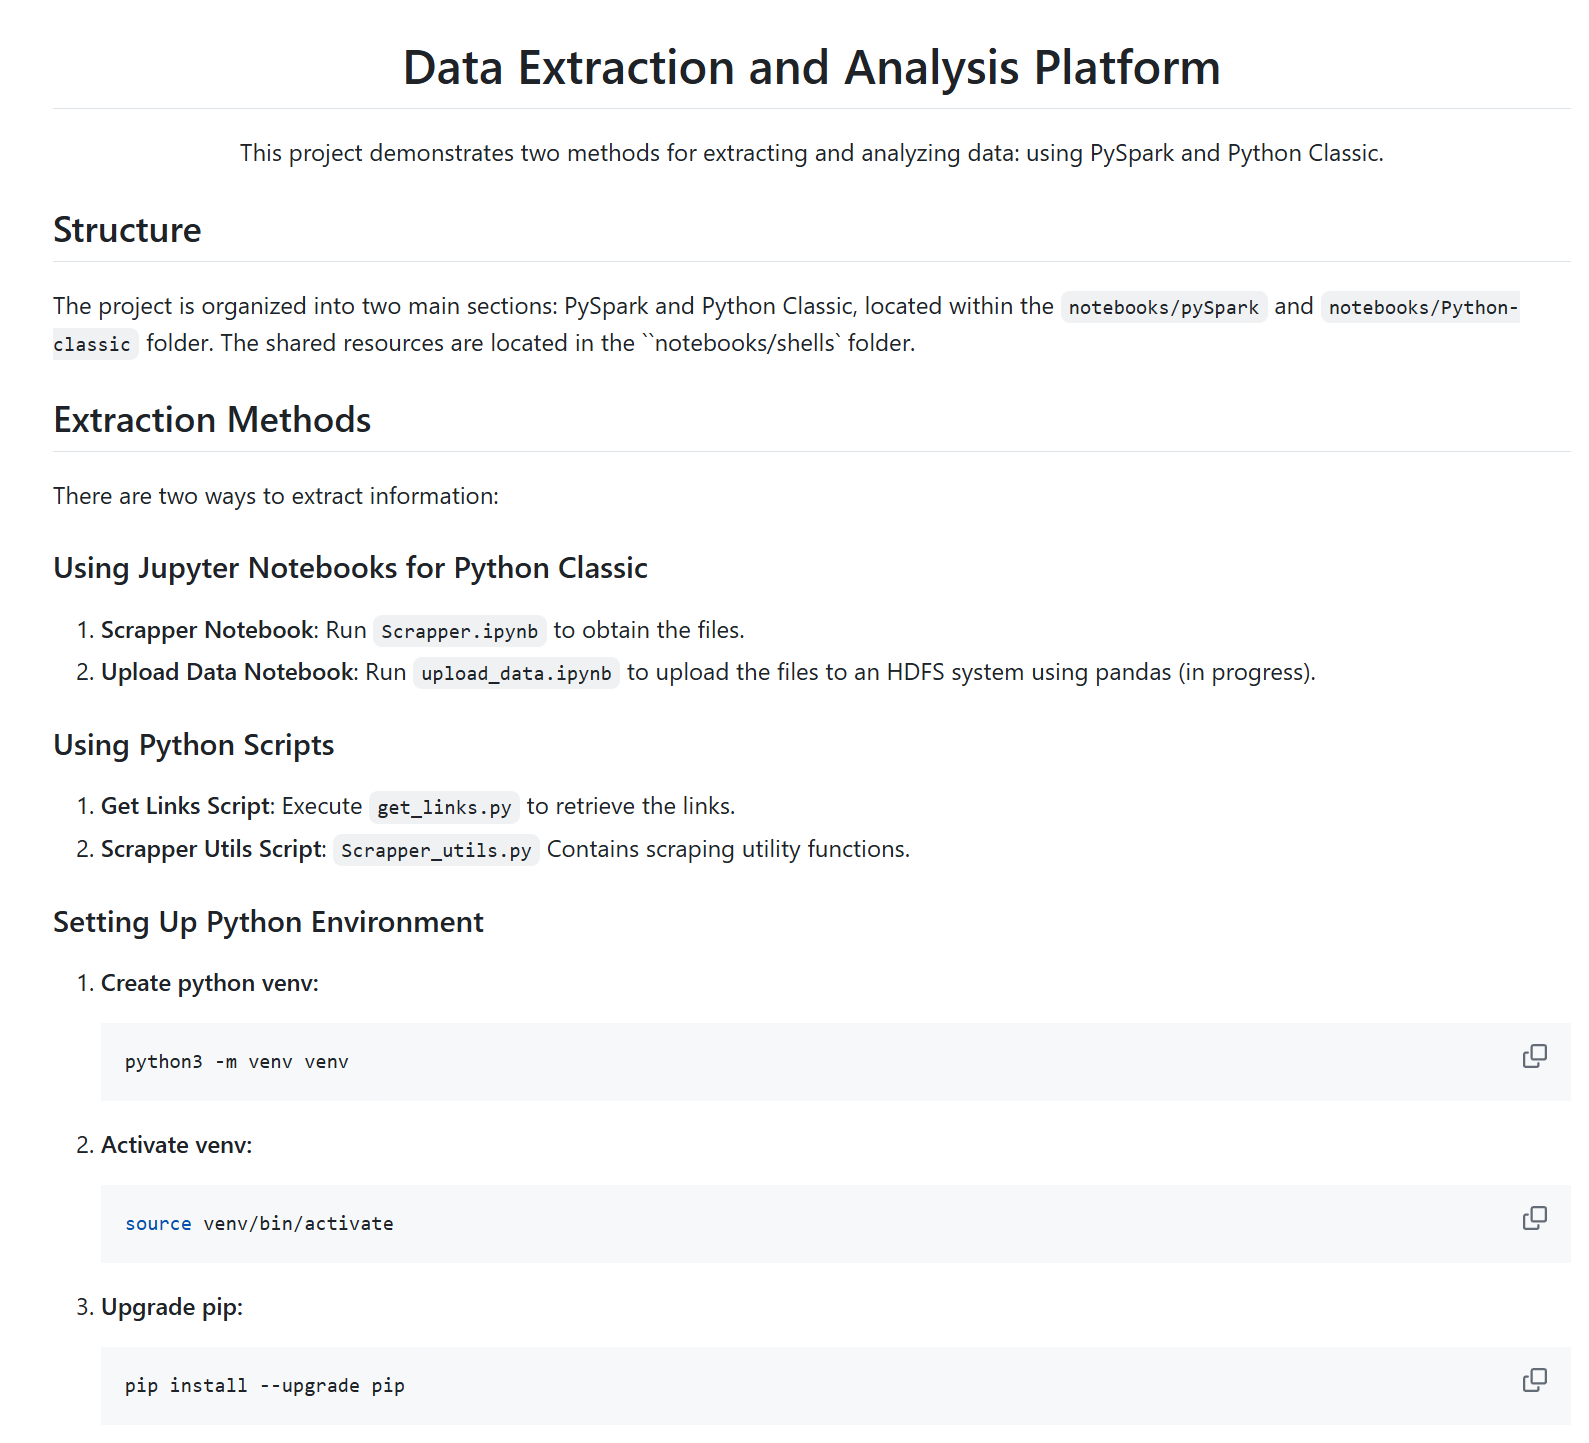
\includegraphics[width=0.6\linewidth]{Reports/images/Extraction.png}
\caption{\label{fig:Extracción}Instrucciones para crear el entorno virtual y extraer los datos de Quién es Quién en los Precios}
\end{figure}

\newpage
Dentro del directorio de \textit{Python classic} podrán encontrar los siguientes archivo adicionales (ver figura 8):

\begin{figure}[h]
\centering
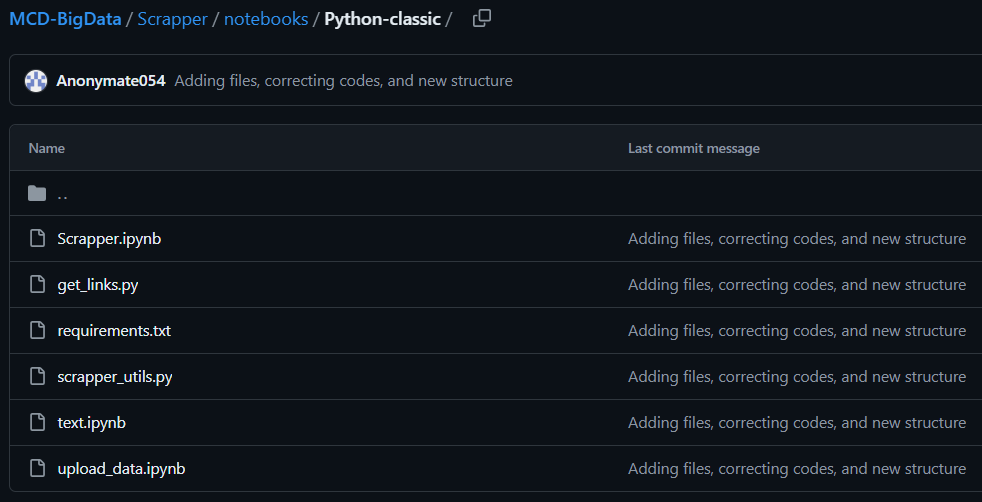
\includegraphics[width=0.3\linewidth]{Reports/images/files.png}
\caption{\label{fig:files}Archivos de configuración}
\end{figure}


Los cuales corresponderán a los archivos de configuración para hacer que el scrapper funcione: \verb|get_links.py|, \verb|scrapper_utils.py| y \verb|text.ipynb|. El archivo \verb|requirements.txt| corresponde a un listado de las bibliotecas y módulos que se requieren para ejecutar el scrapper. 
Por último, el notebook llamado \verb|PySpark-QQP.ipynb| que está en la ruta \textit{Scrapper/notebooks/pySpark/PySpark-QQP.ipynb} es el que contiene los scripts para cargar los datos de cada csv al HDFS usando pyspark. 

\begin{lstlisting}[language=Python]
### Import libraries
from pyspark.sql import SparkSession
from pyspark.sql.functions import lit
from datetime import datetime
from pyspark.sql.types import StructType, StructField, IntegerType, StringType, DecimalType

from IPython.core.display import HTML
display(HTML("<style>pre { white-space: pre !important; }</style>"))

warehouse_location = '/files'

### Create spark session
spark = SparkSession \
    .builder \
    .appName("App de Spark para QQP") \
    .config("spark.sql.warehouse.dir", warehouse_location) \
    .enableHiveSupport() \
    .getOrCreate()

### Print spark info
spark

### List files on hdfs
!hdfs dfs -ls /user/QQP | head -n 6

%%time
!hdfs dfs -count /user/QQP

schema = StructType([
    StructField("PRODUCTO", StringType(), True),
    StructField("PRESENTACIÓN", StringType(), True),
    StructField("MARCA", StringType(), True),
    StructField("CATEGORÍA", StringType(), True),
    StructField("CATÁLOGO", StringType(), True),
    StructField("PRECIO", DecimalType(18, 2), True),
    StructField("FECHAREGISTRO", StringType(), True),
    StructField("CADENACOMERCIAL", StringType(), True),
    StructField("GIRO", StringType(), True),
    StructField("NOMBRECOMERCIAL", StringType(), True),
    StructField("DIRECCIÓN", StringType(), True),
    StructField("ESTADO", StringType(), True),
    StructField("MUNICIPIO", StringType(), True),
    StructField("LATITUD", DecimalType(18, 6), True),
    StructField("LONGITUD", DecimalType(18, 6), True)
])

df = spark.read.csv('/user/QQP/', sep=',', header=False, schema=schema)

# Get the list of input files
file_list = df.inputFiles()
print("Number of input files: ", len(file_list))

%%time
df.count()

%%time
df.count()

### Load data into QQP table
df.write.mode('overwrite').saveAsTable('QQP')

### Close spark session
spark.stop()
\end{lstlisting}

\subsubsection{Extracción, Transformación y Carga (ETL)}

Existe un último proceso que se podría interpretar como un ETL completo, ya que se extraen los datos del HDFS con ayuda del pyspark, se hace realiza un proceso de agregación de datos en el que se seleccionan los productos que corresponden a la canasta básica, se agrupan y agregan mediante la mediana del precio y después se guardan en una tabla en MaríaDB para posteriormente realizar los pronósticos con dicha información.

\begin{lstlisting}[language=Python, caption={python version}]
import warnings
import os   
import pandas as pd
from pyspark.sql import SparkSession
from pyspark.sql.functions import when, col, year, month, countDistinct, avg, stddev, max, min, expr, asc, desc
warnings.filterwarnings("ignore")  

spark = SparkSession.builder \
    .appName("Spark SQL agg") \
    .config("spark.some.config.option", "some-value") \
    .enableHiveSupport() \
    .getOrCreate()

df = spark.read.table('QQP')

df.show(5)

df_agg = df.withColumn(
    "canasta_basica",
    when(
        (col("PRODUCTO") == "ACEITE") & (col("PRESENTACIÓN") == "BOTELLA 946 ML. MIXTO"), 1
    ).when(
        (col("PRODUCTO") == "ARROZ") & (col("PRESENTACIÓN") == "BOLSA 1 KG. SUPER EXTRA"), 1
    ).when(
        (col("PRODUCTO") == "ATUN") & (col("PRESENTACIÓN") == "LATA 140 GR. EN HOJUELAS EN AGUA"), 1
    ).when(
        (col("PRODUCTO") == "AZUCAR") & (col("PRESENTACIÓN") == "BOLSA PLASTICO 2 KG. REFINADA"), 1
    ).when(
        (col("PRODUCTO") == "CARNE RES") & (col("PRESENTACIÓN") == "1 KG. GRANEL. FALDA O PARA DESHEBRAR"), 1
    ).when(
        (col("PRODUCTO") == "CEBOLLA") & (col("PRESENTACIÓN") == "1 KG. BLANCA SIN RABO"), 1
    ).when(
        (col("PRODUCTO") == "CHILE FRESCO") & (col("PRESENTACIÓN") == "1 KG. JALAPEÑO O CUARESMEÑO"), 1
    ).when(
        (col("PRODUCTO") == "CARNE CERDO") & (col("PRESENTACIÓN") == "1 KG. GRANEL. MILANESA O MILANESA DE PIERNA"), 1
    ).when(
        (col("PRODUCTO") == "FRIJOL") & (col("PRESENTACIÓN") == "BOLSA 1 KG. NEGRO"), 1
    ).when(
        (col("PRODUCTO") == "HUEVO") & (col("PRESENTACIÓN") == "PAQUETE CON 12 BLANCO"), 1
    ).when(
        (col("PRODUCTO") == "JABON DE TOCADOR") & (col("PRESENTACIÓN") == "BARRA 180 GR."), 1
    ).when(
        (col("PRODUCTO") == "JITOMATE") & (col("PRESENTACIÓN") == "1 KG. SALADETTE/ HUAJE O TOMATE SALADETTE/ HUAJE"), 1
    ).when(
        (col("PRODUCTO") == "LECHE PASTEURIZADA") & (col("PRESENTACIÓN") == "CAJA 1 LT."), 1
    ).when(
        (col("PRODUCTO") == "LIMON") & (col("PRESENTACIÓN") == "1 KG. AGRIO CON SEMILLA O LIMON COLIMA"), 1
    ).when(
        (col("PRODUCTO") == "MANZANA") & (col("PRESENTACIÓN") == "1 KG. GOLDEN"), 1
    ).when(
        (col("PRODUCTO") == "PIÑA") & (col("PRESENTACIÓN") == "1 KG. O PIÑA ESMERALDA O PIÑA CAYENA"), 1
    ).when(
        (col("PRODUCTO") == "PAN DE CAJA") & (col("PRESENTACIÓN") == "PAQUETE GRANDE 680 GR. REBANADO BLANCO"), 1
    ).when(
        (col("PRODUCTO") == "PAPA") & (col("PRESENTACIÓN") == "1 KG. ALFA/BLANCA"), 1
    ).when(
        (col("PRODUCTO") == "PAPEL HIGIENICO") & (col("PRESENTACIÓN") == "PAQUETE 12 ROLLOS. 200 HOJAS DOBLES"), 1
    ).when(
        (col("PRODUCTO") == "PASTA PARA SOPA") & (col("PRESENTACIÓN") == "PAQUETE 200 GR. SPAGHETTI"), 1
    ).when(
        (col("PRODUCTO") == "CARNE POLLO") & (col("PRESENTACIÓN") == "1 KG. GRANEL. PECHUGA CON HUESO O ANATÓMICA O SIN RABADILLA (CON PIEL)"), 1
    ).when(
        (col("PRODUCTO") == "SARDINA") & (col("PRESENTACIÓN") == "LATA 425 GR. EN TOMATE"), 1
    ).when(
        (col("PRODUCTO") == "TORTILLA DE MAIZ") & (col("PRESENTACIÓN") == "1 KG. GRANEL"), 1
    ).when(
        (col("PRODUCTO") == "ZANAHORIA") & (col("PRESENTACIÓN") == "1 KG. MEDIANA"), 1
    ).otherwise(0)
)

df_agg = df_agg.filter((col("canasta_basica") == 1) & (col("PRECIO").between(5, 1000)))

df_agg = df_agg.groupBy(
    col("FECHAREGISTRO").alias("fecha"),
    year(col("FECHAREGISTRO")).alias("fecha_year"),
    month(col("FECHAREGISTRO")).alias("fecha_month"),
    col("PRODUCTO").alias("producto"),
    col("PRESENTACIÓN").alias("descripcion")
).agg(
    countDistinct("MARCA").alias("count_marca"),
    countDistinct("NOMBRECOMERCIAL").alias("count_tiendas"),
    countDistinct("ESTADO").alias("count_estados"),
    countDistinct("MUNICIPIO").alias("count_municipios"),
    avg("PRECIO").alias("precio_avg"),
    stddev("PRECIO").alias("precio_desv_std"),
    expr("percentile_approx(PRECIO, 0.5)").alias("precio_median"),
    max("PRECIO").alias("precio_max"),
    min("PRECIO").alias("precio_min")
)

df_agg.show()

df_agg.count()

value_counts = df_agg.groupBy("producto").count()
value_counts_sorted = value_counts.orderBy(desc("count"))
value_counts_sorted.show(25)

jdbc_url = "jdbc:mysql://<public-ip>:3306/QQP"
properties = {
    "user": "big_data_user",
    "password": "Example123"
}

df_agg.write.jdbc(url=jdbc_url, table="aggregated", mode="overwrite", properties=properties)

spark.stop()
\end{lstlisting}

\subsection{Análisis Exploratorio de datos}
El análisis exploratorio se describe en el notebook de python llamado \textit{forecast-2.ipynb} y se pued encontrar dentro del github en la siguiente ruta: \href{https://github.com/Anonymate054/MCD-BigData/blob/main/forecast/forecast-2.ipynb}{forecast/forecast-2.ipynb} 


\begin{lstlisting}[language=Python, caption={python version}]

import pandas as pd
import plotly.graph_objects as go
import warnings
from statsmodels.graphics import tsaplots
from utils import extractData_fromMariaDb
import matplotlib.pyplot as plt
warnings.filterwarnings("ignore")

### Load data
df_agg = extractData_fromMariaDb()
df_agg.head()


## Exploratory Data Analysis
### Visualizamos los datos y tambien añadimos bandas para detectar outliers
df_agg["SMA_30"] = df_agg["y"].rolling(window=30).mean()
df_agg["STD_30"] = df_agg["y"].rolling(window=30).std()


df_agg["Upper_Band"] = df_agg["SMA_30"] + (df_agg["STD_30"] * 3)
df_agg["Lower_Band"] = df_agg["SMA_30"] - (df_agg["STD_30"] * 3)

df_agg["Outlier"] = (df_agg["y"] > df_agg["Upper_Band"]) | (df_agg["y"] < df_agg["Lower_Band"])

fig = go.Figure()
fig.add_trace(go.Scatter(x=df_agg["ds"], y=df_agg["y"], mode='lines', name='Datos originales'))
fig.add_trace(go.Scatter(x=df_agg["ds"], y=df_agg["SMA_30"], mode='lines', name='SMA 30 días'))

fig.add_trace(go.Scatter(
    x=pd.concat([df_agg["ds"], df_agg["ds"][::-1]]), 
    y=pd.concat([df_agg["Upper_Band"], df_agg["Lower_Band"][::-1]]),
    fill='toself',
    fillcolor='rgba(0, 176, 246, 0.3)',  
    line=dict(color='rgba(255,255,255,0)'),
    name='Bandas',
    showlegend=False
))


fig.add_trace(go.Scatter(
    x=df_agg[df_agg["Outlier"]]["ds"], 
    y=df_agg[df_agg["Outlier"]]["y"], 
    mode='markers', 
    marker=dict(color='red', size=6),
    name='Outliers'
))


fig.update_layout(
    title='Medias Móviles y Bandas de Desviación Estándar (30 días)',
    xaxis_title='Fecha',
    yaxis_title='Precio Canasta báscia',
    height=800 
)

\end{lstlisting}

Una vez limpiados los datos construimos otro dataframe con los datos limpios, imputamos outliers con SMA y también creamos el date range completo. Se imputan los valores faltantes y se agregan los datos de manera semanal.

\begin{lstlisting}[language=Python, caption={python version}]
df_agg["yclean"] = df_agg["y"]
df_agg.loc[df_agg["Outlier"], "yclean"] = df_agg["SMA_30"]
min_date = df_agg["ds"].min()
max_date = df_agg["ds"].max()

date_range = pd.date_range(start=min_date, end=max_date, freq='D')
df_agg2 = pd.DataFrame(date_range, columns=["ds"])
df_agg2 = df_agg2.merge(df_agg[["ds", "yclean"]], on="ds", how="left")

## imputamos los nulos generado al completar el date range
rolling_mean = df_agg2['yclean'].rolling(window=5, min_periods=1).mean()
df_agg2['yclean'] = df_agg2['yclean'].combine_first(rolling_mean.shift())
df_agg2.rename(columns={'yclean': 'y'}, inplace=True)
df_agg2.head(20)

## agregamos los datos de manera semanal
df_agg2['y'] = pd.to_numeric(df_agg2['y'], errors='coerce')

df_agg2.set_index('ds', inplace=True)
df_weekly = df_agg2.resample('W').mean().reset_index()
df_weekly.head(20)

\end{lstlisting}

Revisamos nuestro diagrama de autocorrelación para las pruebas de estacionariedad. 

\begin{lstlisting}[language=Python, caption={python version}]
df_weekly["SMA_4"] = df_weekly["y"].rolling(window=4).mean()
df_weekly["STD_4"] = df_weekly["y"].rolling(window=4).std()

df_weekly["Upper_Band"] = df_weekly["SMA_4"] + (df_weekly["STD_4"] * 3)
df_weekly["Lower_Band"] = df_weekly["SMA_4"] - (df_weekly["STD_4"] * 3)

fig = go.Figure()

fig.add_trace(go.Scatter(x=df_weekly["ds"], y=df_weekly["y"], mode='lines', name='Datos originales'))
fig.add_trace(go.Scatter(x=df_weekly["ds"], y=df_weekly["SMA_4"], mode='lines', name='SMA 4 semanas'))


fig.add_trace(go.Scatter(
    x=pd.concat([df_weekly["ds"], df_weekly["ds"][::-1]]), 
    y=pd.concat([df_weekly["Upper_Band"], df_weekly["Lower_Band"][::-1]]),
    fill='toself',
    fillcolor='rgba(0, 176, 246, 0.5)', 
    line=dict(color='rgba(255,255,255,0)'),
    name='Bandas',
    showlegend=False
))

fig.update_layout(
    title='Medias Móviles y Bandas de Desviación Estándar (4 semanas)',
    xaxis_title='Fecha',
    yaxis_title='Precio Canasta Básica (Semanal)',
    height=800 
)

fig.show()
\end{lstlisting}

,y vemos el resultado (ver figura 9)

\begin{figure}[h]
\centering
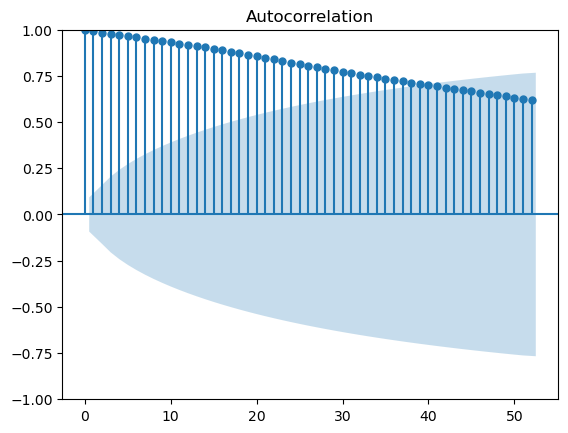
\includegraphics[width=0.65\linewidth]{Reports/images/auto.png}
\caption{\label{fig:auto}Diagrama de autocorrelación}
\end{figure}

\newpage
\subsection{Pronósticos}

Por último, en la generación delos pronósticos se usaron bibliotecas como Prophet y media móviles. Después de hacer evaluaciones de el modelo podemos obtener los siguiente resultados de la figura 10.

\begin{figure}[h]
\centering
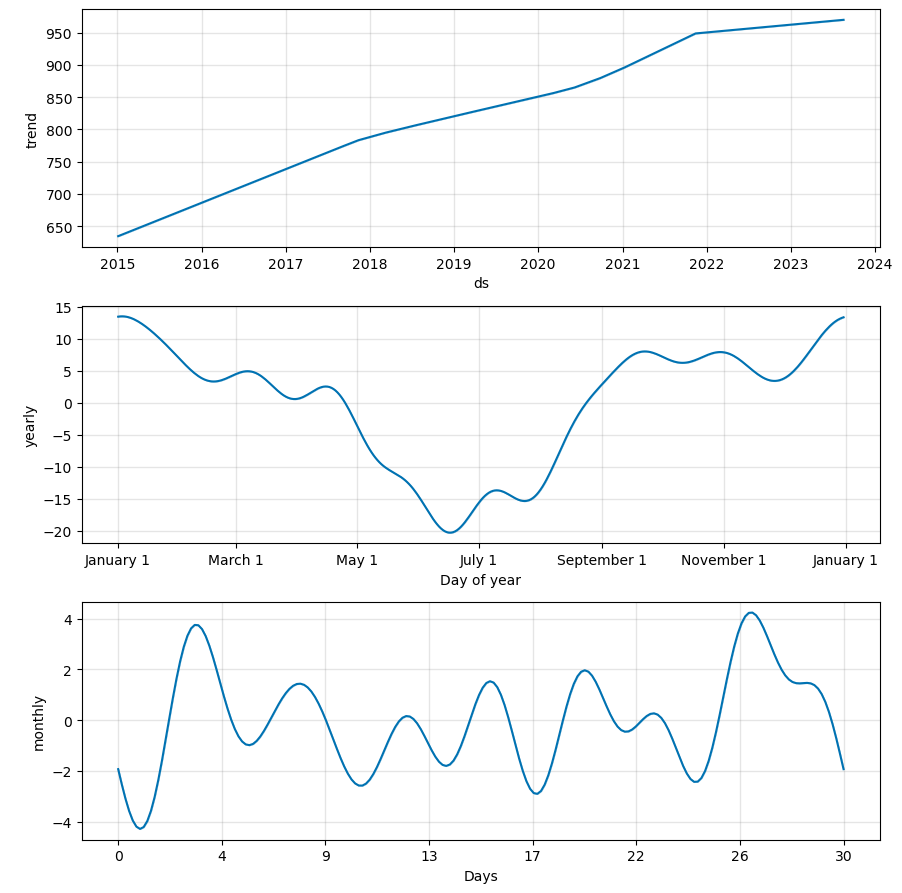
\includegraphics[width=0.8\linewidth]{Reports/images/trend.png}
\caption{\label{fig:trend}Análisis de series de tiempo}
\end{figure}

\newpage
Finalmente obtuvimos los pronósticos siguientes (ver figura 11). 

\begin{figure}[h]
\centering
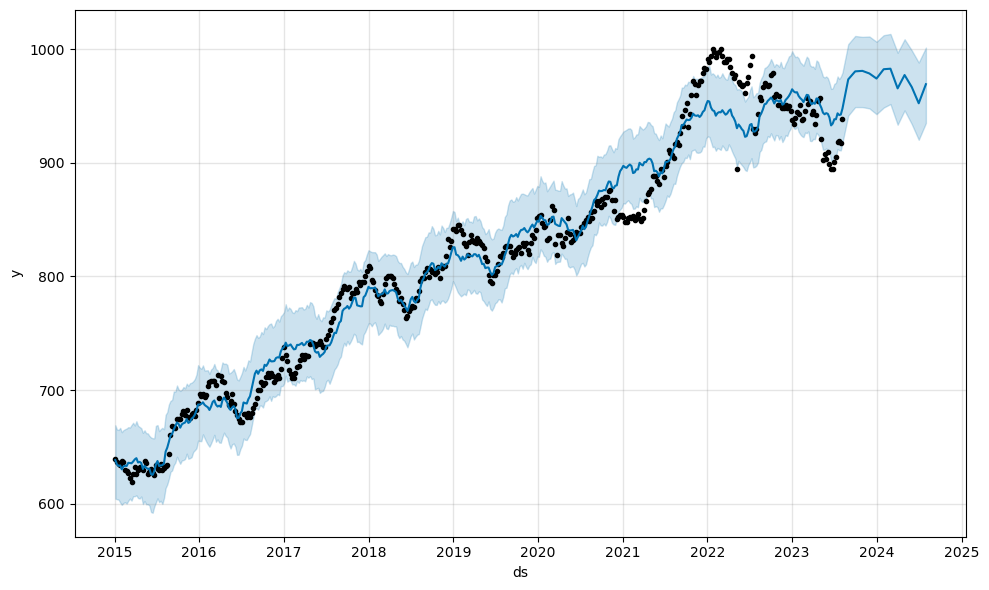
\includegraphics[width=0.9\linewidth]{Reports/images/pronostico.png}
\caption{\label{fig:pronostico} Ajuste del modelo y pronóstico de precios}
\end{figure}

Un tema importante a considerar, es que mientras más amplio sea el horizonte de predicción, la precisión del modelo decrecerá, puesto que los precios siguen dependiendo de las fluctuaciones del mercado y común mente no es posible predecir cómo se podría comportar la demanda de un producto en especifico. Sin embargo, el objetivo es brindar pronósticos de una o dos semanas en el futuro, por lo que el resultado sigue siendo una buena referencia acerca de cómo podrían cambiar los precios de los productos.


\begin{figure}[h]
\centering
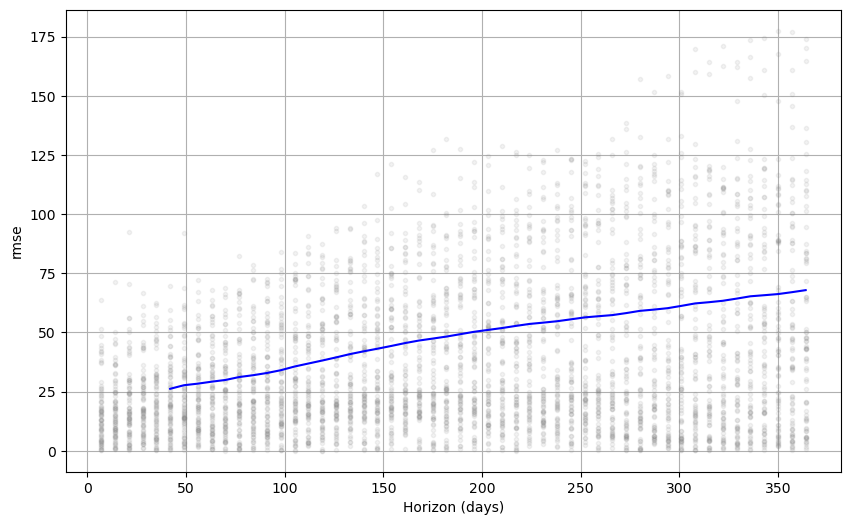
\includegraphics[width=0.7\linewidth]{Reports/images/predict.png}
\caption{\label{fig:Architecture}Predicción}
\end{figure}


\newpage
\subsubsection{Arquitectura de solución completa}
A continuación se muestra la arquitectura creada para este proyecto.

\begin{figure}[h]
\centering
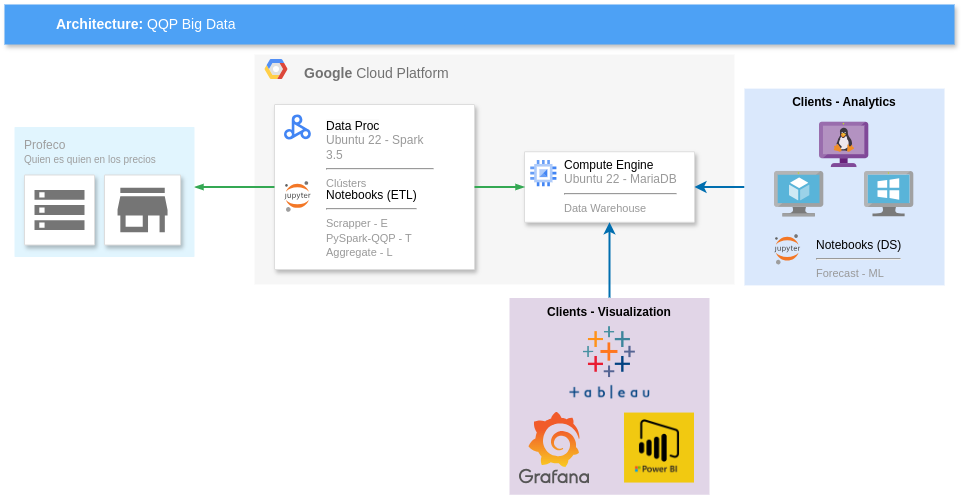
\includegraphics[width=0.7\linewidth]{images/Architecture_QQP_BD.png}
\caption{\label{fig:Architecture}Arquitectura de solución}
\end{figure}

Consta de una instancia de Dataproc, con la instalación de un sistema linux con PySpark. En dicha instancia es donde se extrae, se carga y se transforma la información. Posteriormente se manda la tabla agregada a otra instancia que cuenta con una base de datos de MariaDB, la cual permite que otros usuarios pueda acceder a la información de forma rápida y eficiente. \\

Finalmente mediante esta infraestructura se pueden conectar tanto clientes de analítica (como es el caso del análisis Forecast) como de visualizaciones que se podrían generar a partir de la información obtenida.

\section{Resultados y Conclusiones}

El enfoque de grandes datos en la creación de este proyecto fue bueno. A pesar de no haber podido hacer un sistema que se actualizara en tiempo real, se cumplió con la creación de un proceso que extrae los datos y que se puede actualizar conforme se sube la información a la página. Si en algún momento QPP quisiera subir los datos por día, nuestro sistema lograría actualizar la información con esa misma rapidez.

\section{Trabajos a futuro}

Actualmente se está trabajando en mejorar los scripts y códigos para automatizar las tareas del análisis. Especialmente los corresponden a la creación de la infraestructura en la nube. Posteriormente se considerará explorar realizar una imagen de un contenedor que cuenta con toda la configuración hecha para sólo levantarse. \\

Por otro lado, la actualización de los archivos por parte de PROFECO indican que se realizan cada 6 meses. Por lo que es se puede generar una alerta o una función que únicamente tome los nuevos archivos para incorporarlos al sistema y correr un nuevo reentrenamiento. \\

Durante el proceso, se identificó que existen herramientas serverless que permiten realizar las  mismas actividades, pero presuntamente a un menor costo. Por lo que será importante considerarlo para las mejoras.\\

Finalmente generar un sistema que permita visualizar la información de forma rápida y efectiva, como podría ser Grafana, Power Bi o Talbeau. Así como, levantar un servicio API REST que permite interconectar el modelo con otros sistemas. 

% \bibliographystyle{alpha}
% \bibliography{sample}

\end{document}